\chapter{Estado del Arte}\label{chapter:state-of-the-art}

\section{\textit{Big data} y telefonía} 

El crecimiento sostenido de la población humana, junto con su concentración en áreas urbanas y el aumento de su movilidad, ha planteado retos significativos para la adaptación de los sistemas sociales y demográficos. Estas dinámicas impactan directamente en la planificación y desarrollo de políticas públicas, ya que entender los patrones de movilidad resulta crucial para abordar problemas en diversas áreas. Por ejemplo, en la planificación del transporte, conocer cómo se desplazan las personas permite diseñar redes de carreteras más eficientes y sistemas de transporte público mejor adaptados a las necesidades de la población. En el ámbito de la salud, el modelado de la propagación de enfermedades infecciosas se beneficia de estos datos, ya que facilita la implementación de restricciones y controles más efectivos. Además, en el sector comercial, el geomarketing utiliza los patrones de movilidad para optimizar la distribución geográfica de publicidad y anuncios, maximizando su impacto \cite{asgari2013survey}.

Históricamente, el análisis de la movilidad humana se basaba en métodos tradicionales como encuestas, observación directa o censos poblacionales. Aunque útiles, estos enfoques presentan limitaciones significativas debido a su elevado costo, frecuencia limitada y dependencia de muestras pequeñas, lo que dificulta obtener una visión integral de los flujos de movilidad \cite{asgari2013survey}. En las últimas décadas, el desarrollo tecnológico ha permitido explorar nuevas fuentes de datos. Algunos estudios como \cite{gong2012gps} hacen uso de los sistemas GPS, que ofrecen una alta precisión en exteriores, sin embargo su uso puede ser intermitente debido al consumo de batería de los dispositivos, y por lo general requieren de la instalación de software específico y la activación del mismo por parte del usuario. Esto implica que los estudios basados en GPS suelan estar limitados a pequeñas muestras. Una alternativa, menos precisa pero mucho más abarcadora, es el uso de datos provenientes de las redes de telecomunicaciones, en particular los registros generados por los teléfonos móviles. Estos dispositivos, que actualmente son utilizados por el 80$\%$ de la población mundial mayor de 10 años y hasta el 90$\%$ en regiones como América y Europa \cite{ITU2024}, recopilan una cantidad masiva de datos vinculados a la actividad de sus usuarios \cite{toole2015path} que se requieren para el correcto funcionamiento de la red.

Los registros de telefonía móvil incluyen información como la identificación anónima del usuario, la ubicación de las radio bases con las que interactúan sus dispositivos y marcas temporales, permitiendo rastrear trayectorias de movilidad en tiempo real. Esto convierte a los teléfonos móviles en una plataforma de censado masivo de la actividad humana \cite{doyle2014population}, que no solo es económica y escalable, sino también capaz de proporcionar una visión general de los desplazamientos individuales y colectivos. Estas trayectorias ofrecen información valiosa para el análisis de la movilidad humana, contribuyendo a la toma de decisiones en múltiples campos y representando un recurso crucial para la investigación y el desarrollo de soluciones basadas en datos.

\subsection*{Registros de Telefonía Móvil}

Una red de telefonía celular se compone de una infraestructura de radio desplegada en áreas denominadas celdas, cada una equipada con al menos una estación base transmisora-receptora fija (BTS, por sus siglas en inglés, \textit{base transceiver station}) \cite{sharma2012cell}. Estas estaciones permiten establecer conexiones inalámbricas entre los terminales de los usuarios y la red en cualquier momento. Las interacciones generadas entre los dispositivos móviles y las BTS se almacenan en registros que contienen información clave, como identificadores de los usuarios y de las estaciones a las que se conectan \cite{yuan2013characterizing}. La estructura y el tipo de registros generados pueden variar según la tecnología utilizada por el proveedor de la red, aunque ciertos estándares han sido adoptados de manera general \cite{durive2021sistema}.

Entre los registros de mayor interés para estudios de movilidad se encuentran los Call Detail Records (CDR) y los Location Update Records (LUR) \cite{gutierrez2020como}. Los CDR se generan durante eventos específicos, como llamadas, mensajes o conexiones a la red, y son comúnmente utilizados para la facturación de los usuarios, lo que asegura su almacenamiento por largos períodos. Estos registros incluyen información como identificadores de los dispositivos, marcas de tiempo y tipos de eventos, siendo ampliamente utilizados en estudios de movilidad gracias a su disponibilidad. Por otro lado, los LUR son activados por la red en situaciones como cambios de cobertura o períodos de inactividad, proporcionando una mayor resolución temporal al registrar eventos independientes de las actividades de los usuarios. Sin embargo, debido a que no son utilizados para facturación, suelen ser desechados, lo que limita su aplicación en estudios de movilidad \cite{durive2021sistema}.

A pesar de las diferencias en los eventos que generan estos registros, ambos comparten una estructura de información similar, incluyendo identificadores, eventos, celdas y marcas temporales. Estos datos permiten aproximar las localizaciones de los usuarios en diferentes momentos, aunque la resolución espacial depende de la densidad de las BTS, la cual varía significativamente entre áreas urbanas y rurales \cite{forghani2020cellular}. Al identificar registros con el mismo identificador de usuario, es posible reconstruir trayectorias aproximadas que muestran las posiciones de las estaciones base a las que un dispositivo se conectó mientras se desplazaba \cite{chen2018individual}. En este contexto, una colección de trayectorias derivadas de datos de telefonía móvil puede ofrecer una representación aproximada de la movilidad.

\subsection*{Desafíos}

Los datos de redes de telecomunicaciones han revolucionado los estudios de movilidad humana al proporcionar grandes volúmenes de información que superan las limitaciones de métodos tradicionales como las encuestas. Aunque estos datos han abierto nuevas posibilidades para investigar patrones de movilidad, también presentan desafíos significativos.

Uno de los principales retos es garantizar la privacidad de los usuarios, la cual ha recibido mucha atención en los años recientes. La protección de información sensible ha llevado a restricciones en el acceso a los registros, incluso cuando están anonimizados. Por ejemplo en \cite{tesselkin2017estimation} se presenta un modelo de red de transporte en forma de cadena de Markov para la estimación de las matrices origen-destino (O-D). Con cierta similitud, en \cite{pourmoradnasseri2019od} un modelo de Markov de segundo orden es empleado bajo la premisa de investigar patrones de movilidad humanos a partir de telefonía celular. Resultando de interés, en particular, la determinación de matrices O-D y el completamiento de trayectoria.

A pesar de los avances, el balance entre el aprovechamiento de los datos y la protección de la privacidad sigue siendo una barrera crítica en la investigación, especialmente en contextos donde el acceso a datos es fundamental para obtener resultados significativos.

\subsection*{Historia en Cuba}

La Empresa de Telecomunicaciones de Cuba, Etecsa, es la única empresa en el territorio nacional que provee servicios de telefonía móvil e Internet. A pesar de grandes avances los últimos años, estos servicios demoraron más tiempo para hacerse populares y accesibles a la mayor parte de la población cubana respecto a la media mundial \cite{durive2021sistema}. Como consecuencia directa, la experiencia con el uso de datos de la red de telefonía celular para estudios de movilidad en Cuba esta limitada a años recientes.

Según se relata en \cite{durive2021sistema}, en 2018 comienza un esfuerzo por parte de investigadores del actual Centro de Sistemas Complejos de la Facultad de Física de la Universidad de La Habana para acceder a los registros de telefonía celular con el objetivo de extraer analítica que enriqueciera los procesos de toma de decisiones por parte de las autoridades de salud, planificación del transporte y estudios socio-demográficos, etc. Obteniéndose el acceso a registros de tipo LUR a partir del año 2020, acordándose con Etecsa la firma de un acuerdo de confidencialidad con la universidad y el compromiso de respetar una serie de métodos de seguridad entre los que figura que:

\begin{itemize}
    \item los datos de LUR son almacenados en servidores de Etecsa, dentro de la red de la compañía;
    \item los datos son almacenados sin identificadores de usuarios, como nombre, teléfono o IMSI;
    \item ningún dato de granularidad individual puede sustraerse de la red de la empresa;
    \item ningún procedimiento de ingeniera inversa o \textit{de-anonymization} puede usarse;
    \item los datos se entregan con fines de investigación y solo pueden usarse para estos fines;
    \item Etecsa emite por escrito autorización para la divulgación de los resultados obtenidos.
\end{itemize}

Etecsa ha desplegado más de 1,500 radiobases en Cuba, con una distribución heterogénea que refleja la densidad de usuarios, concentrándose en áreas urbanas. Para proteger la ubicación precisa de estas torres, se adoptó una estrategia que agrupa torres cercanas en zonas densas y ajusta ligeramente su posición en zonas rurales, reduciendo el número a 795 pseudo-torres con ubicaciones GPS compartidas. Estas pseudo-torres se emplean en estudios de movilidad mediante zonas de cobertura definidas con celdas de Voronoi, funcionando de manera similar a las torres reales para los análisis realizados.

El estudio de la movilidad poblacional a partir de los registros LUR de la empresa Etecsa está amparado por la legislación cubana. En particular la Ley de protección de Datos Personales \cite{cuervo2022resolucion}, del 2022, define lo que se consideran datos personales (que incluye los datos generados por sistemas tecnológicos como los teléfonos) y las reglas para su uso. Estipula que dichos datos pueden usarse por razones de bienestar general si se someten previamente a un procedimiento de disociación, como el antes mencionado.

El valor social de comprender y usar estos datos quedó demostrado ampliamente cuando en medio de la pandemia de SARS-CoV2 a partir de marzo de 2020, el sistema de salud y el gobierno cubanos pudieron disponer de modelos de movilidad para evaluar la efectividad de las medidas de limitación de movimiento que se implementaron. Es importante resaltar que, durante ese mismo período, la mayor parte de los gobiernos del mundo usaron métricas semejantes para entender la epidemia y sus consecuencias. En muchos casos, los modelos de movilidad provinieron de empresas como Google, que amparada por la urgencia médica mundial, puso a disposición de los investigadores modelos de movilidad basados en la detección de posicionamiento de los usuarios a partir de los metadatos generados por sus aplicaciones. Es de señalar que Google excluyó a Cuba de la lista de países que podían acceder a dichos datos, como se muestra en la figura \ref{fig:google_exclusion}.

\begin{figure}[!htb] \centering 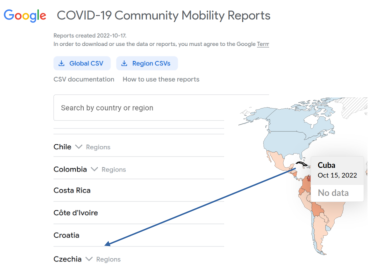
\includegraphics[width=0.5\textwidth]{Graphics/google_exclusion.pdf} \caption{Cuba excluida por Google en el acceso a datos de movilidad} \label{fig:google_exclusion} \end{figure}

Si bien los modelos de movilidad generados por el Centro de Sistemas Complejos, de acuerdo con Etecsa, fueron de gran utilidad, es importante señalar que dichos datos tienen menos precisión y menos abundantes que los que disponen empresas como Google, Facebook y otras.

Una de las enseñanzas de la pandemia y de la posterior aplicación de estos datos al estudio de la movilidad poblacional es que no se puede esperar a tener situaciones críticas para decidirse a usar estos métodos de \textit{big data}. Esencialmente, aunque el posible uso y valor de estos datos sea bastante obvio, en los detalles de cómo extraer valor informacional radica un gran reto. Es importante crear una base científica y tecnológica que permita, ante necesidades concretas, saber las potencialidades de estos datos, si permiten o no enfrentar la tarea en cuestión, y la precisión de los mismos.

\section{Antecedentes}

El completamiento de trayectorias, ha recibido especial atención debido a las limitaciones relacionadas con la resolución temporal y espacial de los registros de telefonía móvil. Se ha presentado un amplio grupo de metodologías orientadas hacia este problema, frecuentemente uniendo datos de telefonía con la estructura de alguna red de transporte. Contando estas metodologías con un grupo de limitaciones.

Se pueden encontrar algunas metodologías de completamiento basadas en interpolación, como el caso de \cite{hoteit2014estimating}. La interpolación, en general, es precisa cuando la densidad de puntos es elevada, lo cual no suele ser el caso de los registros de telefonía, además de que no suele usar información de trayectorias similares para el completamiento. De forma similar \cite{st2014reconstructing} realiza el completamiento uniendo nodos para lograr el camino más corto dentro de una red de tránsito a la cual son mapeadas las localizaciones de los registros y Vajakas et al. \cite{vajakas2015trajectory} propone un completamiento basado en asignar el camino mas rápido entre los dos puntos de la red de tránsito de la cual se tengan registros consecutivos.

Por su parte, \cite{chen2019complete} utiliza la periodicidad en la movilidad humana y la factorización de tensores para completar trayectorias individuales, para lo cual se necesitan datos de un mismo usuario por un largo período de tiempo. Otros trabajos orientados al completamiento de trayectorias complementan los registros con información topológica \cite{forghani2020cellular} o información sobre el \textit{handoff} entre torres \cite{derrmann2019road}.

El marco GRFTrajRec \cite{zhaograph} aborda los desafíos de datos de trayectorias urbanas de baja frecuencia mediante una innovadora representación basada en grafos que integra dimensiones de red y trayectoria. Con un modelo seq2seq sensible a intervalos espaciotemporales, este enfoque logra capturar atributos esenciales en los puntos de trayectoria, permitiendo restaurar puntos GPS ausentes con alta precisión.

Una buena parte de los trabajos orientados al completamiento de trayectorias de movilidad utilizan técnicas de aprendizaje automático o redes neuronales artificiales (ANN, por \textit{artifcial neural network}). Por ejemplo, en \cite{partsinevelos2005reconstructing} se presenta una métodología para reconstruir trayectorias a partir de imágenes, utilizando una ANN para refinar las trayectorias después de una etapa de \textit{clustering}. Zhang et al. \cite{zhang2019prnet} propone una red neuronal profunda combinando redes convolucionales, secuenciales y dos mecanismos de atención para estimar localizaciones en exteriores a partir de información de la red de telefonía que incluye datos de la intensidad de la señal del usuario respecto a diferentes torres. La trayectoria se reconstruye a partir de las localizaciones estimadas a partir de una técnica de \textit{map-matching} presentada en \cite{zheng2014urban}.

% \section{Modelos de movilidad}

% \subsection{Reconstruccion de trayectorias}

\section{Aprendizaje automático}

El aprendizaje automático abarca diversas técnicas y modelos que permiten a las computadoras aprender y tomar decisiones a partir de datos. Los principales paradigmas del aprendizaje automático son tres: \textbf{aprendizaje supervisado}, \textbf{aprendizaje no supervisado} y \textbf{aprendizaje por refuerzo}. En esta sección, se presenta una base teórica para la comprensión del primero de estos enfoques, el aprendizaje supervisado vinculado con el análisis de secuencias.

El aprendizaje supervisado es uno de los métodos más utilizados en el aprendizaje automático. En este enfoque, los modelos se entrenan utilizando datos etiquetados, es decir, conjuntos de datos en los que cada entrada está emparejada con su salida correcta. Durante el proceso de aprendizaje, el modelo genera predicciones basadas en los datos de entrada y las compara con las salidas reales. La diferencia entre las predicciones y las salidas correctas, medida a través de una función de pérdida, guía el ajuste de los parámetros internos del modelo. A través de iteraciones sucesivas, este proceso permite al modelo aprender un mapeo efectivo entre las entradas y las salidas, mejorando su precisión para predecir casos nuevos no incluidos en los datos de entrenamiento, siempre y cuando se logre una correcta generalización del aprendizaje.

En el ámbito del aprendizaje supervisado se identifican principalmente dos categorías de problemas: clasificación y regresión. Mientras que la clasificación se enfoca en la predicción de categorías discretas, asignando entradas a determinadas etiquetas, la regresión, por otro lado, aspira a prever valores continuos. En esta esfera del conocimiento, varias técnicas han prevalecido, siendo algunas de las más renombradas los árboles de decisión \cite{breiman2017classification}, máquinas de vectores de soporte (SVM) \cite{cortes1995support}, K-vecinos más próximos (K-NN) \cite{cover1967nearest}, Naive Bayes \cite{john2013estimating} y, notablemente, las Redes Neuronales Artificiales \cite{chollet2021deep}.

\subsection{Redes neuronales}

Las redes neuronales han sido un pilar fundamental en el desarrollo del aprendizaje automático, transformando múltiples áreas de investigación y aplicaciones prácticas, incluyendo la visión por computadora, el procesamiento del lenguaje natural (PNL) y, más recientemente, la predicción y completamiento de trayectorias humanas. Inspiradas en el funcionamiento del cerebro humano (McCulloch \& Pitts, 1943), las redes neuronales han evolucionado desde los primeros perceptrones hasta arquitecturas complejas como las redes multicapa (MLP) y el aprendizaje profundo. Sin embargo, las arquitecturas tradicionales presentan limitaciones significativas al abordar tareas que involucran secuencias temporales complejas o relaciones contextuales a largo plazo.

Por ejemplo, las redes convolucionales (CNNs), que han demostrado ser altamente efectivas en el procesamiento de datos estructurados como imágenes (LeCun et al., 1998), no están diseñadas para capturar la información temporal inherente a las secuencias. Las redes recurrentes (RNNs), por otro lado, introducen la capacidad de procesar información temporal mediante un flujo recurrente de datos (Elman, 1990). A pesar de sus avances, las RNNs enfrentan problemas como el desvanecimiento y la explosión del gradiente (Hochreiter, 1991), lo que dificulta su capacidad para aprender dependencias a largo plazo. Las variantes como las LSTMs (Hochreiter \& Schmidhuber, 1997) y GRUs (Cho et al., 2014) intentaron mitigar estos problemas mediante puertas de control, pero aún se encuentran limitadas en términos de eficiencia computacional y escalabilidad para secuencias largas.

\subsection{\textit{Embeddings}}

En el aprendizaje automático, los \textit{embeddings} son representaciones densas y de baja dimensión de datos, diseñadas para capturar relaciones semánticas y estructurales entre elementos en un espacio continuo. Estas representaciones han revolucionado áreas como el Procesamiento del Lenguaje Natural (PLN) y la visión por computadora al transformar datos categóricos o de alta dimensión en vectores manejables por modelos.

Un \textit{embedding} es un vector numérico que representa un objeto, como una palabra, imagen o usuario, en un espacio donde las relaciones geométricas reflejan relaciones significativas en los datos originales \cite{bengio2000neural}. Por ejemplo, en el caso del lenguaje, palabras con significados similares estarán cerca en el espacio de los \textit{embeddings}.

En términos matemáticos, un \textit{embedding} transforma un elemento discreto $x$ (como una palabra o un ID) en un vector $\mathbf{v} \in \mathbb{R}^n$, donde $n$ es la dimensionalidad del espacio.

\subsubsection*{Importancia}

\begin{itemize}
    \item \textbf{Reducción de dimensionalidad}: Representan datos categóricos de alta dimensión en espacios densos y continuos.
    \item \textbf{Eficiencia computacional}: Reducen el costo computacional frente a representaciones dispersas como la codificación \textit{one-hot}.
    \item \textbf{Captura de semántica}: Modelan relaciones implícitas en los datos, como similitud semántica o relaciones gramaticales.
\end{itemize}

\subsubsection*{Aplicaciones Principales}

\begin{itemize}
    \item \textbf{Procesamiento del Lenguaje Natural}:
    Los \textit{embeddings} de palabras, como \textit{Word2Vec} \cite{mikolov2013efficient} y \textit{GloVe} \cite{pennington2014glove}, han sido fundamentales para tareas como traducción automática y análisis de sentimientos.

    \item \textbf{Sistemas de Recomendación}:
    Representan usuarios y elementos (por ejemplo, películas o productos) en el mismo espacio, permitiendo encontrar correspondencias cercanas basadas en similitudes de \textit{embeddings}.

    \item \textbf{Visión por Computadora}:
    En redes convolucionales (CNN), las capas intermedias generan \textit{embeddings} de imágenes que capturan características visuales. Estos \textit{embeddings} se usan para tareas como clasificación y búsqueda visual \cite{krizhevsky2012imagenet}.

    \item \textbf{Modelado de Grafos}:
    Los \textit{embeddings} de nodos, como en \textit{Node2Vec} \cite{grover2016node2vec}, representan la estructura y conectividad de grafos, facilitando tareas como predicción de enlaces y clasificación de nodos.
\end{itemize}

En resumen, los \textit{embeddings} son herramientas esenciales en el aprendizaje automático moderno, permitiendo que los modelos trabajen de manera eficiente con datos complejos y categóricos, capturando relaciones profundas entre los elementos representados.

\subsection{Atención}

El mecanismo de atención es un avance clave en la inteligencia artificial, inspirado en el proceso humano de enfocarse en información relevante mientras se ignora lo superfluo. Este concepto, ampliamente utilizado en aprendizaje automático, permite que los modelos asignen recursos computacionales de manera efectiva y se concentren en las partes más importantes de los datos.

Introducido por Bahdanau et al. \cite{bahdanau2014neural}, el mecanismo de atención marcó un hito en el diseño de modelos neuronales para tareas de secuencias. Resolviendo un desafío crítico de las redes recurrentes, permite manejar dependencias a largo plazo en secuencias largas, donde la información temprana tiende a desvanecerse debido al problema del gradiente. En arquitecturas tradicionales como las RNNs y LSTMs, esta limitación obstaculizaba el aprendizaje eficiente en datos extensos.

Por su diseño, la atención redefine la forma en que los modelos procesan secuencias al asignar pesos dinámicos a los elementos de entrada según su relevancia para el resultado actual. En términos simples, permite que el modelo ``preste atención'' de manera diferenciada a diferentes partes de la secuencia, en lugar de procesarlas de manera uniforme. Este enfoque no solo mejora la retención de información importante, sino que también permite que los modelos procesen secuencias de forma más efectiva. Matemáticamente, la atención se define como una combinación ponderada de todas las representaciones de entrada. Los pesos de atención se calculan utilizando una función de compatibilidad que evalúa cuán bien se alinean las representaciones de entrada con la representación de salida en un paso dado.

\subsubsection*{Componentes}

El mecanismo de atención estándar consta de tres componentes principales:

\begin{enumerate}
    \item \textbf{Consultas, claves y valores (Q, K, V)}:
    La entrada se proyecta en tres espacios de representación diferentes: consultas (\(Q\)), claves (\(K\)) y valores (\(V\)). Estas proyecciones se obtienen mediante transformaciones lineales con parámetros aprendibles. Las consultas representan el contexto actual, las claves codifican las características de las entradas, y los valores contienen la información que será combinada de acuerdo a los pesos calculados.

    \item \textbf{Función de compatibilidad}:
    Para calcular los pesos de atención, se evalúa la similitud entre cada consulta (\(Q\)) y las claves (\(K\)) correspondientes. Comúnmente, se utiliza el producto punto escalado, definido como:
    \[
    \text{Compatibilidad}(Q, K) = \frac{QK^\top}{\sqrt{d_k}},
    \]
    donde \(d_k\) es la dimensión de las claves, y la escala \(\sqrt{d_k}\) estabiliza los gradientes.

    \item \textbf{Pesos de atención}:
    Los pesos se calculan aplicando la función softmax sobre los resultados de la función de compatibilidad, asegurando que los valores sean no negativos y sumen uno. Esto permite interpretar los pesos como una distribución de probabilidad sobre las entradas.

    \item \textbf{Combinación ponderada}:
    Los valores (\(V\)) se combinan mediante una suma ponderada utilizando los pesos calculados. El resultado final es una representación contextualizada de las entradas, enfocada en los elementos más relevantes.
\end{enumerate}

\subsubsection*{Atención Multi-Cabeza}

Vaswani et al. \cite{vaswani2017attention} expandieron el mecanismo de atención estándar al introducir la \textbf{atención multi-cabeza} en la arquitectura Transformer. En lugar de calcular una única representación contextual, el modelo divide las representaciones de consultas, claves y valores en múltiples subconjuntos de menor dimensionalidad y calcula diferentes pesos de atención en paralelo. Esto permite que cada cabeza de atención capte distintos aspectos de las relaciones entre los elementos de la secuencia.

Formalmente, en la atención multi-cabeza:
\[
\text{head}_i = \text{Attention}(QW_i^Q, KW_i^K, VW_i^V),
\]
donde \(W_i^Q\), \(W_i^K\), y \(W_i^V\) son matrices de proyección aprendibles para la \(i\)-ésima cabeza. Las salidas de todas las cabezas se concatenan y se proyectan de vuelta al espacio original mediante otra transformación lineal.

\subsubsection*{Beneficios del Mecanismo de Atención}

El mecanismo de atención presenta múltiples ventajas clave que lo hacen superior a enfoques tradicionales:
\begin{itemize}
    \item \textbf{Paralelización}: A diferencia de las RNNs, la atención permite procesar todos los elementos de la secuencia simultáneamente, lo que mejora significativamente la eficiencia computacional.
    \item \textbf{Flexibilidad}: Los pesos de atención no están restringidos a la posición en la secuencia, lo que permite capturar relaciones contextuales a largas distancias.
    \item \textbf{Generalización}: La atención es adaptable a diferentes tipos de datos, como texto, imágenes y trayectorias, haciendo que los modelos basados en atención sean altamente versátiles.
\end{itemize}

En resumen, el mecanismo de atención no solo revolucionó el aprendizaje de secuencias, sino que también sentó las bases para el desarrollo de arquitecturas más eficientes y potentes, consolidándose como una herramienta indispensable en el aprendizaje automático moderno.

\subsection{BERT}

BERT (\textit{Bidirectional Encoder Representations from Transformers}) es un modelo avanzado para el procesamiento de secuencias, introducido por Devlin et al. en 2018 \cite{devlin2018bert}. Basado en la arquitectura Transformer \cite{vaswani2017attention}, BERT destaca por su capacidad de capturar relaciones contextuales en ambas direcciones (izquierda-derecha y derecha-izquierda) dentro de una secuencia.

Una de las características principales de BERT es su enfoque bidireccional, que se implementa mediante el mecanismo de atención \cite{vaswani2017attention}. Este enfoque permite procesar simultáneamente la información contextual en toda la secuencia. Las capas de codificadores (\textit{encoders}) del Transformer facilitan esta operación al representar cada elemento de la secuencia como una combinación ponderada de los demás elementos, capturando así relaciones globales y locales en la secuencia.

El método de preentrenamiento de BERT es clave para su rendimiento y se basa en dos tareas principales:

\begin{itemize}
    \item \textbf{Máscara de elementos (\textit{Masked Language Model}, MLM):} Durante el entrenamiento, se enmascaran aleatoriamente algunos elementos de la secuencia de entrada, y el modelo debe predecirlos en función del contexto restante. Este enfoque obliga al modelo a comprender el contexto completo, tanto a nivel local como global, en cualquier tipo de secuencia.
    
    \item \textbf{Predicción de relaciones (\textit{Next Sentence Prediction}, NSP):} Aunque esta tarea es más relevante en problemas textuales, también refuerza la capacidad del modelo para identificar patrones de relación entre diferentes segmentos de una secuencia.
\end{itemize}

Gracias a su arquitectura bidireccional, BERT es especialmente eficaz para abordar problemas donde las dependencias dentro de las secuencias son intrínsecamente bidireccionales y donde el orden de los elementos influye significativamente en su relación contextual.



% y eso se ve en detalle en el capitulo siguiente
